\documentclass[a2paper, 12pt]{article}
\usepackage[font={huge, bf}]{caption}
\usepackage{fontspec}
\setmainfont{Arial}
\usepackage{subcaption}
\usepackage{graphicx}
\usepackage{tikz}
\usepackage{tikzsymbols}
\usetikzlibrary{calc,patterns,shapes.geometric}
\usepackage{float}
\usepackage{pdflscape}
\usepackage{geometry}
\geometry{landscape, margin=2cm}
\captionsetup[subfigure]{justification=justified,singlelinecheck=false}
\pagestyle{empty}

\def\centerarc[#1](#2)(#3:#4:#5){\draw[#1] ($(#2)+({#5*cos(#3)},{#5*sin(#3)})$) arc (#3:#4:#5);}

\begin{document}
	\vspace*{\fill}
	\begin{figure}[!htbp]
		\centering
		\begin{subfigure}[b]{0.48\textwidth}
			\caption{Figure 1}
			\centering
			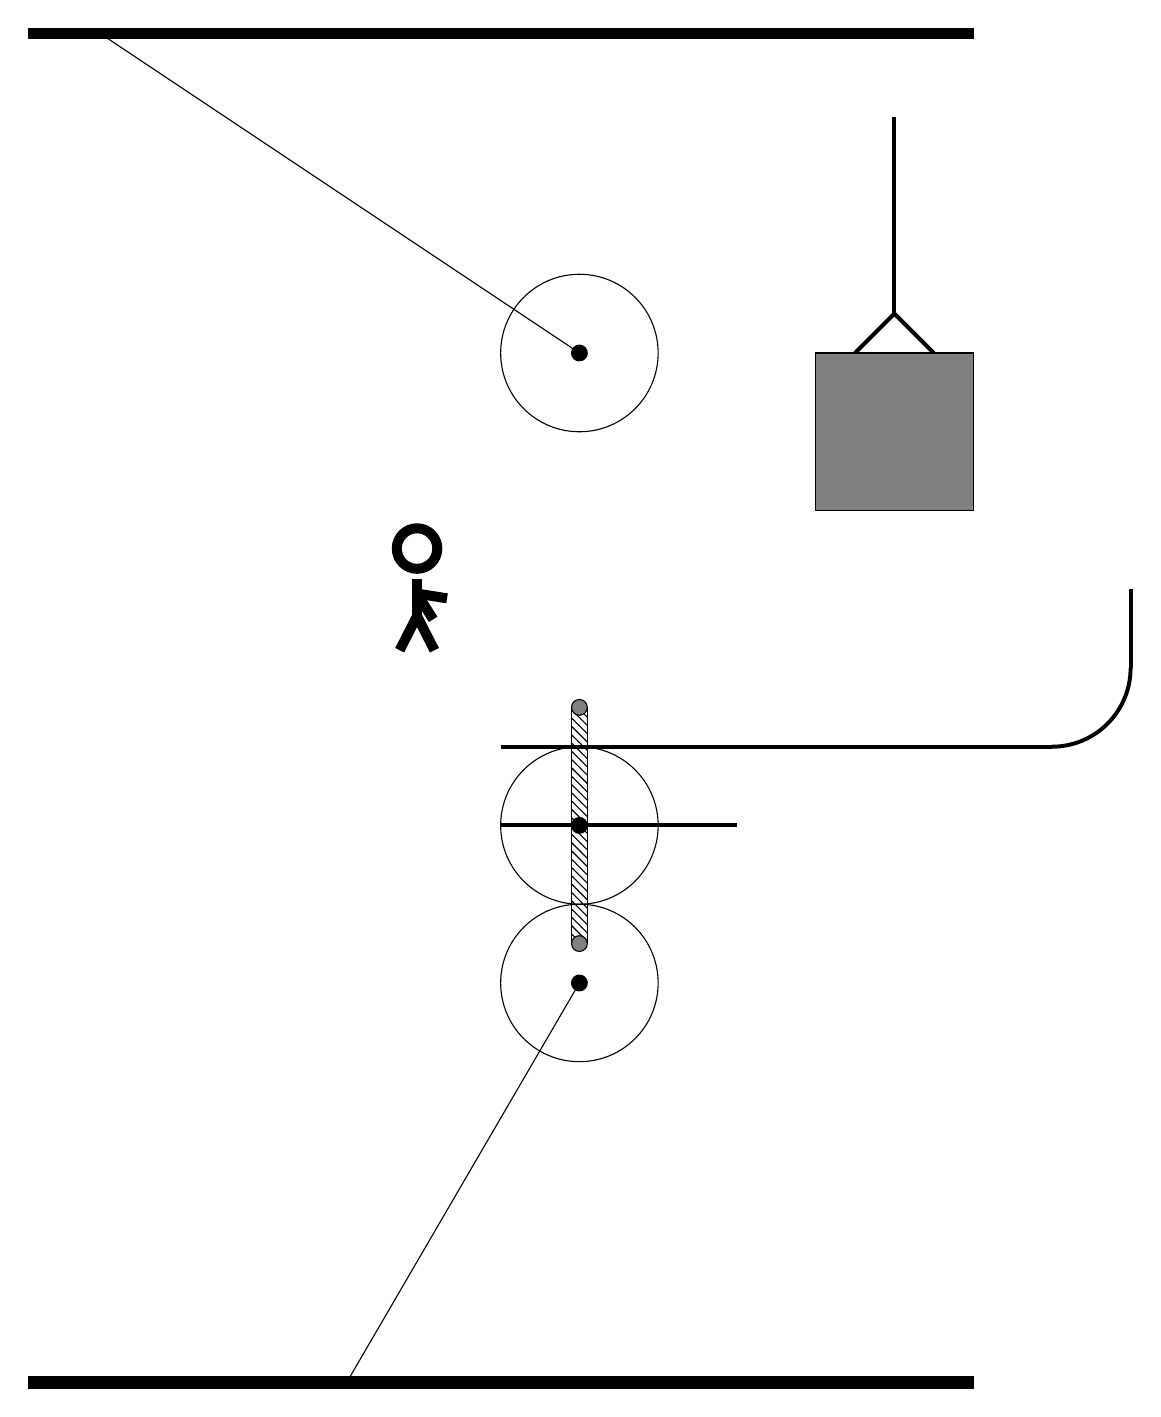
\begin{tikzpicture}
				\draw[fill=black] (-6, 14) rectangle (6, 14.125);
				
				\draw (1,10) circle (1);
				\draw[fill=black] (1,10) circle (0.1);
				\draw (-5,14.0) -- (1,10);
				
				\draw (1,4) circle (1);
				\draw[fill=black] (1,4) circle (0.1);
				\draw[pattern=north west lines, pattern color=black] (0.9,5.5) rectangle (1.1,2.5);
				\draw[fill=black!50] (1,5.5) circle (0.1);
				\draw[fill=black!50] (1,2.5) circle (0.1);
				
				\draw (1,2) circle (1);
				\draw[fill=black] (1,2) circle (0.1);
				\draw (-2,-3.15) -- (1,2);
				
				\draw[line width=0.5mm](5,10.5) -- (5,13.0);
				\draw[line width=0.5mm](4.5,10) --  (5,10.5) -- (5.5,10);
				\draw[fill=black!50] (4, 10) rectangle (6, 8);
				
				\draw[line width = 0.5mm] (0,5) -- (7,5);
				\draw[line width = 0.5mm] (7,5) arc (270:360:1);
				\draw[line width = 0.5mm] (8,6) -- (8,7);
				\draw[line width = 0.5mm] (0,4) -- (3,4);
				\centerarc[line width = 0.5mm](0,3)(90:180:1);
				
				\node at (-1, 7) {\scriptsize \Strichmaxerl[10][122][-9]};
				
				\draw[fill=black] (-6, -3) rectangle (6, -3.15);
			\end{tikzpicture}
		\end{subfigure}
		\hfill
		\begin{subfigure}[b]{0.48\textwidth}
			\caption{Figure 2}
			\centering
			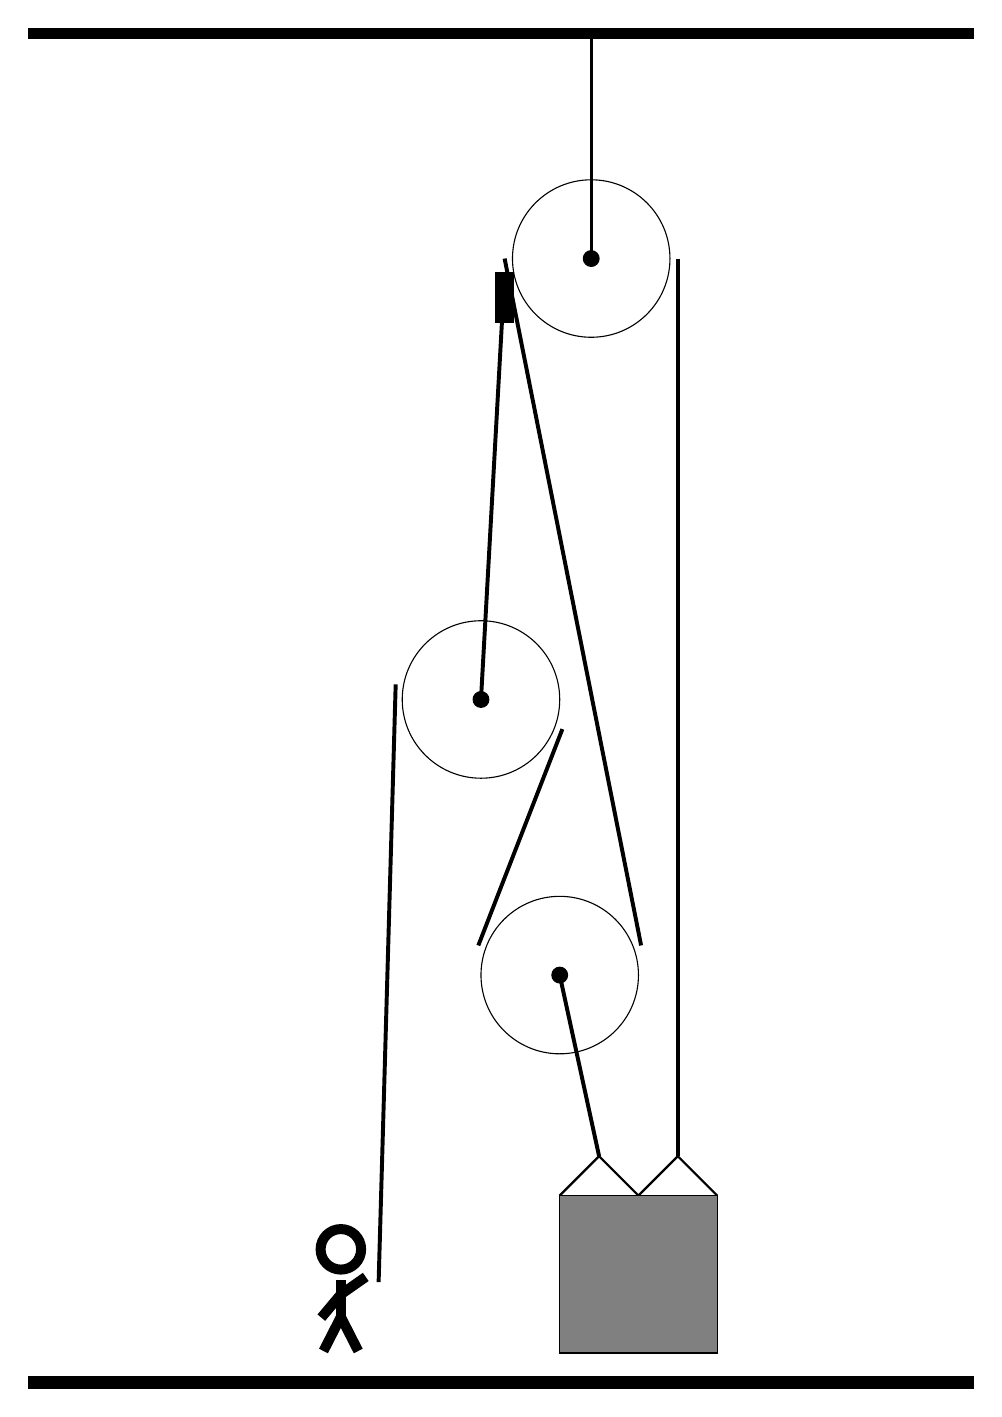
\begin{tikzpicture}
				\draw[fill=black] (-6, 14) rectangle (6, 14.125);
				
				\draw (-0.25, 5.6) circle (1);
				\draw[fill=black] (-0.25, 5.6) circle (0.1);
				
				\draw (0.75, 2.1) circle (1);
				\draw[fill=black] (0.75, 2.1) circle (0.1);
				
				\draw (1.15, 11.2) circle (1);
				\draw[fill=black] (1.15, 11.2) circle (0.1);
				\draw[very thick] (1.15, 11.2) -- (1.15, 14);
				
				\draw[thick]  (0.75, -0.7) -- (1.25, -0.2) -- (1.75, -0.7) -- (2.25, -0.2) -- (2.75, -0.7);
				\draw[fill=black!50] (0.75, -0.7) rectangle (2.75, -2.7);
				
				\draw[line width=0.5mm] (-0.25, 5.6) -- (0.05, 11.0);
				\draw[line width=0.5mm, fill=black](-0.05, 10.4) rectangle (0.15, 11.0);
				\draw[line width=0.5mm] (-1.55, -1.8) -- (-1.3333, 5.791);
				\centerarc[line width=0.5mm](-0.25, 5.6)(-20:170:1.1);
				\draw[line width=0.5mm] (0.7837, 5.2238) -- (-0.2837, 2.4762);
				\centerarc[line width=0.5mm](0.75, 2.1)(160:380:1.1);
				\draw[line width=0.5mm] (1.7837, 2.4762) -- (0.05, 11.2);
				\draw[line width=0.5mm](0.75, 2.1) -- (1.25, -0.2);
				\centerarc[line width=0.5mm](1.15, 11.2)(0:180:1.1);
				\draw[line width=0.5mm] (2.25, 11.2) -- (2.25, -0.2);
				
				\node at (-2, -1.9) {\scriptsize \Strichmaxerl[10][50][35]};
				
				\draw[fill=black] (-6, -3) rectangle (6, -3.15);
			\end{tikzpicture}
		\end{subfigure}
	\end{figure}
		\vspace*{\fill}
\end{document}